\chapter{SysML Case Study}\label{sysml}
The following chapter introduces a real world example of the \ac{UML} profile
\ac{SysML} in a detailed manner. At first an
introduction of the case study is given considering the semantics of the corresponding models.
Afterwards the case study is analyzed regarding technical and pragmatical issues
and their relevance related to modeling tools. This chapter lays the foundation
for chapter~\ref{solution}, in which the presented case study is used as exemplary input.
\section{Introduction}\label{sysml:introduction}
A real world case study concerning the domain of systems engineering presented by
the technical university of Munich in~\cite{aiscasestudy} has been modeled in
\ac{SysML}, as this \ac{UML} profile has been developed with such domain in
mind. The case study is evolved around a \ac{PPU}, which can be described as an
industrial automation plant. Its main purpose is the processing of given
elements like metallic pieces by picking them up and placing them onto a slide.
This scenario lays the foundation for the following revisions of this case
study and is depicted in figure~\ref{ppu_rev0}. The whole case study pursues
the target of demonstrating different iterations of a real world automation
\ac{PPU}, whereas the developers of this plant will add, remove or edit
elements throughout the revisions.

Revision 1, as shown in figure~\ref{ppu_rev1}, adds a new \textit{Y-Slide} to
the \ac{PPU} which will replace the simple slide of revision 0 and has to be
integrated into the semantics of the crane additionally for example. Now the
\ac{PPU} fills up both parts of this new slide as it increases the capacity for
work pieces. This is just a small example of the changes between each revision, a
more in-depth look at all revision changes can be taken in
the appendix~\ref{appendix:sysml_casestudy} or in the
publication~\cite{aiscasestudy}.

\begin{figure}[h!]
\begin{center}
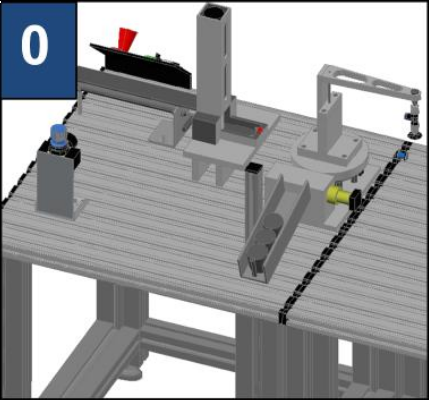
\includegraphics[scale=0.4]{ppu_rev0}\\
\end{center}
\caption{\ac{PPU} case study revision 0~\cite{aiscasestudy}}
\label{ppu_rev0}
\end{figure}

The case study itself consists of 14 consecutive revisions each representing a
new version of the \ac{PPU} consisting of changes made by the developers.
The scope and the differences between each revision is
presented in figure~\ref{revisionChanges_analysis}: Revision 0 consists of
approximately 550 elements which are corresponding to revision 1
for example. As depicted via the blue graph, elements are mostly added which
finally leads to 1216 correspondences between revision 12 and 13. Noticeable
peaks of differences and therefore corresponding operations between revision 2
and 3 as well as 4 and 5 can be explained by the semantics of the changes: The
first peak corresponds to a new \textit{Stamp} module, which adds a
lot of new elements with its own semantics to the \ac{PPU} for example.

\begin{figure}[h!]
\begin{center}
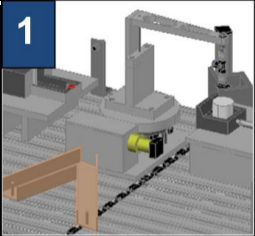
\includegraphics[scale=0.6]{ppu_rev1}\\
\end{center}
\caption{\ac{PPU} case study revision 1~\cite{aiscasestudy}}
\label{ppu_rev1}
\end{figure}

Figure~\ref{revisionChanges_analysis} is the result of the combined usage of
all tools and services implemented as part of this Master's Thesis, whereas the results
themselves are presented in chapter~\ref{solution}.

\begin{figure}[h!]
\begin{center}
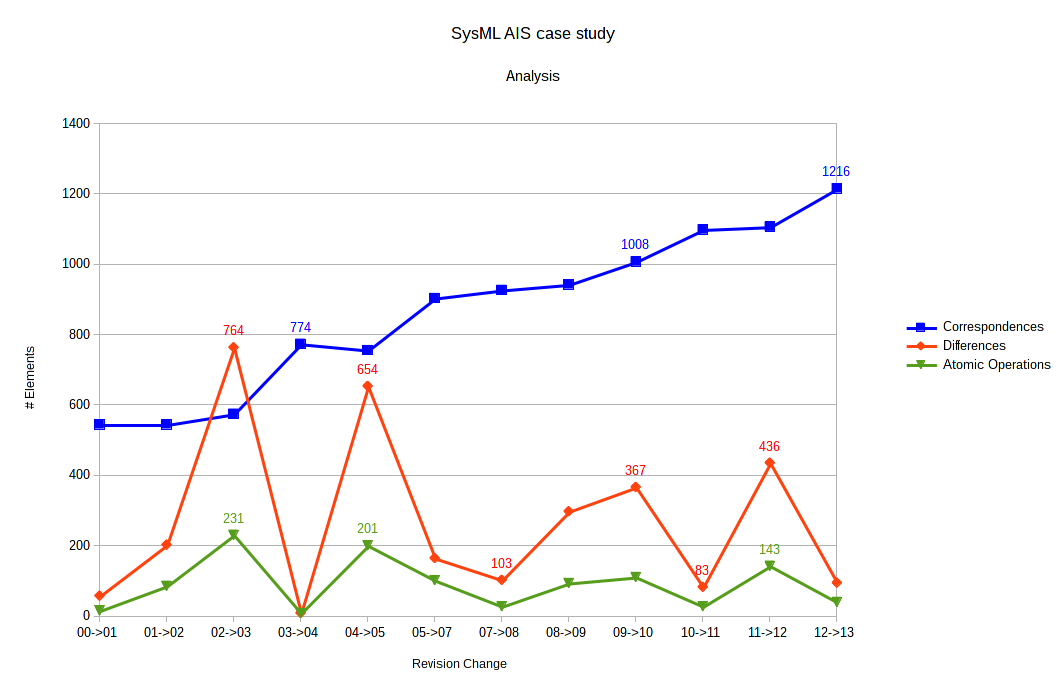
\includegraphics[scale=0.5]{revisionChanges_analysis}\\
\end{center}
\caption{\ac{PPU} revision changes overview}
\label{revisionChanges_analysis}
\end{figure}

\section{Analysis}\label{sysml:analysis}
Additionally to the semantics explained in the previous section, the \ac{SysML}
case study has been analyzed in detail regarding issues of different variants.
Several tools have been developed as part of this analysis, which shall not be
explained in this Master's Thesis as only their results are of importance. Three
types of issues have been defined, as they differ in impact on modeling tools and will be explained hereafter.

 \textbf{Technical Issues}\\
 Issues of this type have a crucial impact on modeling tools, as the results
 may differ distinguishably in absence of such issues. Whereas some modeling
 tools may deliver slighty wrong results, other modeling tools may deliver
 substantial wrong ones. Three examples of such issues found in the \ac{PPU}
 shall be given:
 \begin{itemize}
   \item \textbf{Wrong \ac{UUID}s}\\
   		 The example of
		 wrong \ac{UUID}s already given in figure~\ref{wrongUUIDs_examples_p3} shall
	 	 be recalled: The \ac{UUID}s of two corresponding associations in consecutive
	 	 revisions of the \ac{PPU} differ, as the association in the later revision
	 	 has been created newly by the developer. They describe the same semantics
	 	 thus both associations should be matched and the only change detected should
	 	 be a name change of the association. As many modeling tools rely on correct
	 	 identifiers, they would produce wrong results which differ extremely from
	 	 the expected. A summary of all wrong \ac{UUID}s found through all revisions
	 	 of this \ac{SysML} case study is shown in figure~\ref{wrongUUIDs_summary}.
	 	 The red bars are describing \textit{newly} created \ac{UUID} mismatches
	 	 between revisions, whereas the green bars present the number of wrong
	 	 identifiers carried over from older revisions.
	 	 	 	
		\begin{figure}[h!]
		\begin{center}
		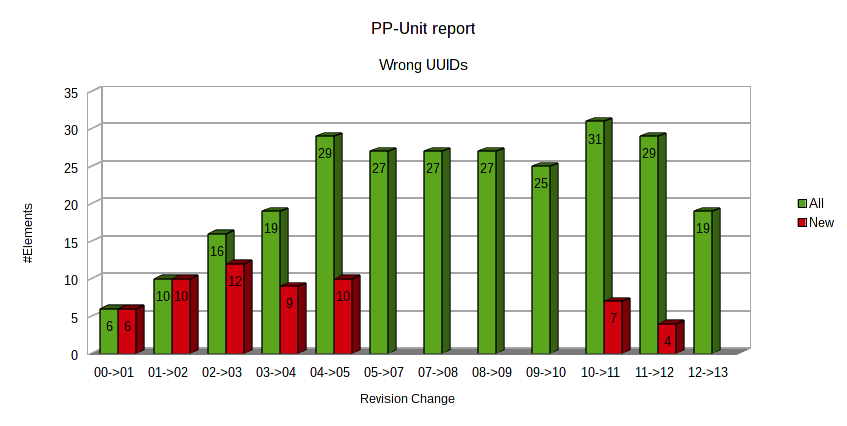
\includegraphics[scale=0.6]{wrongUUIDs}\\
		\end{center}
		\caption{Summary of wrong \ac{UUID}s}
		\label{wrongUUIDs_summary}
		\end{figure}
		
  \item \textbf{Usage of EAnnotations}\\
  		\textit{EAnnotations} are available in Ecore models for annotating modeling
  		elements. They are defined like every other modeling element, therefore are
  		also considered during the detection of differences and correspondences
  		between models if absent. The case study is modeled in \ac{SysML} using
  		Papyrus\cite{PapyrusURL}, which will create EAnnotations for internal usage
  		of representation of associations as illustrated in
  		figure~\ref{eannotations}. Separating visual elements from semantic elements
  		is crucial in all areas of software development, especially in the case of
  		\ac{MDSD}. This is an example which problems can be caused if such
  		requirements are not met by modeling tools: Differencing between
  		two revisions which have been created with different tools will lead to
  		wrong results, as the EAnnotations added by Papyrus will cause differences.
  		\begin{figure}[h!]
		\begin{center}
		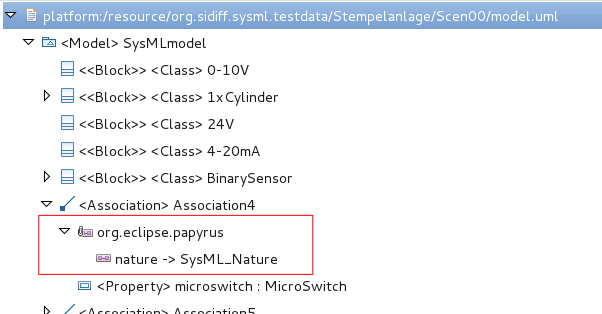
\includegraphics[scale=0.4]{eannotations}\\
		\end{center}
		\caption{EAnnotations created by Papyrus}
		\label{eannotations}
		\end{figure}
		
	\item \textbf{Usage of special characters}\\
		\ac{UML} does support the usage of special characters, which may
		cause problems in used modeling tools. Each modeling tool may handle these
		characters differently, as they may escape them with new ones or do not alter
		them at all. An example of the usage of such special characters can be
		depicted in listing~\ref{specialcharacter_example}: Papyrus itself escaped the
		character \glqq <\grqq\  by using the equivalent \glqq \&lt;\grqq\ whereas
		the opposite character \glqq >\grqq\ is not altered at all. These problems
		may cause problems at saving or loading the models, as the special characters
		are interpreted differently depending on the used modeling tool.
		
	\lstset{ language=XML,
    caption={Example of special character usage},
    morekeywords={xmi:type, xmi:id,name,encoding, basePackage, stereoPackage},
    label=specialcharacter_example
    }	
		    \begin{lstlisting}
 <subvertex xmi:type="uml:State" name="&lt;&lt;InCycle>>PickedUpState">
 	<doActivity xmi:type="uml:OpaqueBehavior" name="WPPickedUp:=TRUE;"> 
 		<language>Natural language</language>
 		<body>Kran_Sauger_an:=FALSE;&#xD; Kran_Sauger_aus:=true;</body>
  </doActivity>
 </subvertex>\end{lstlisting}
 \end{itemize}
 
\textbf{Pragmatical Issues}\\
This type of issues can be described as pragmatical, as they are not affecting
modeling tools and their result themselves but may lead to wrong understanding
of models by the developer. As described earlier, the \ac{SysML} case study has
been created using Papyrus, which makes use of its own diagram format. It
separates the view onto the models via its different diagrams from the
underlying model and offers the possibility to \textit{hide} modeling elements, which are
still present in the model itself. Unaware of consequences using this feature,
developers may hide elements in a particular revision, followed by another
developer not knowing of their existence in the model. This leads
to different pragmatical issues which have been categorized as follows:
	
\begin{itemize}
  \item \textbf{Missing elements}\\
  
\begin{figure}[h!]
\begin{center}
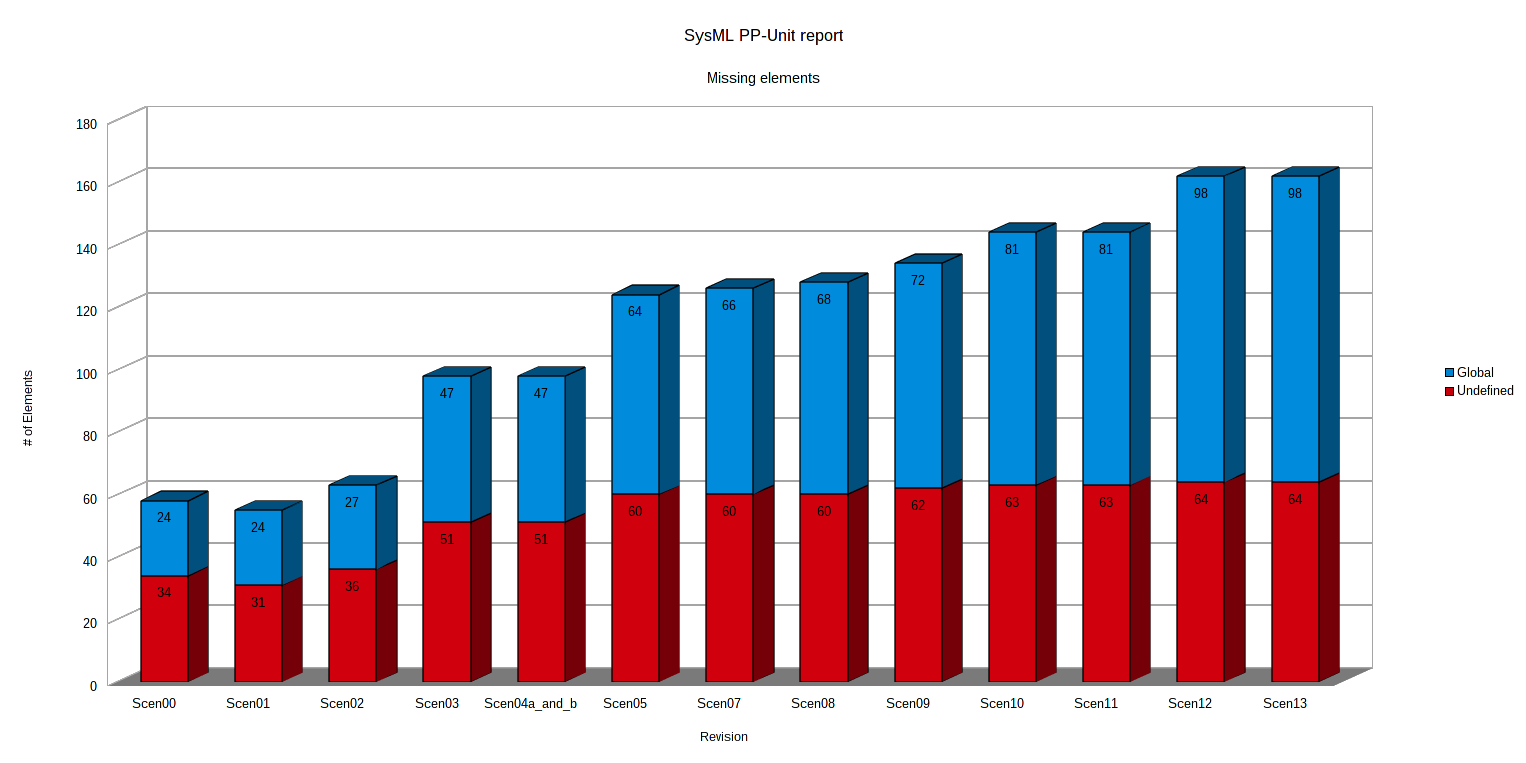
\includegraphics[scale=0.35]{missingElements}\\
\end{center}
\caption{Missing elements summary}
\label{missingElements}
\end{figure}
  		As mentioned before, hiding elements in a particular diagram view may lead
  		to the misunderstanding, that these elements do not exist within the model
  		itself. As shown in figure~\ref{missingElements}, there have been defined
  		two types of such elements:
  		\begin{itemize}
  		  \item[\underline{Undefined elements}] have to be defined in at least one
  		  diagram, for that the developer must know of their existence without the need of using
  		  other viewers as the diagram view itself. This category of elements has
  		  been further divided as depicted in figure~\ref{undefinedElementTypes}.
  		  Modeling elements described as undefined are important as they may change
  		  the understanding the model drastically. Examples of such elements are
  		  \textit{Block} or \textit{State}.
  		  
  		  \item[\underline{Global elements}] do not need to be defined in at least
  		  one diagram, as they are expected to be declared globally. This
  		  declaration can be imagined to be implemented outside of the given model,
  		  as these include elements such as \textit{Constraint} or \textit{Literal}.
  		\end{itemize}
	\begin{figure}[h!]
	\begin{center}
	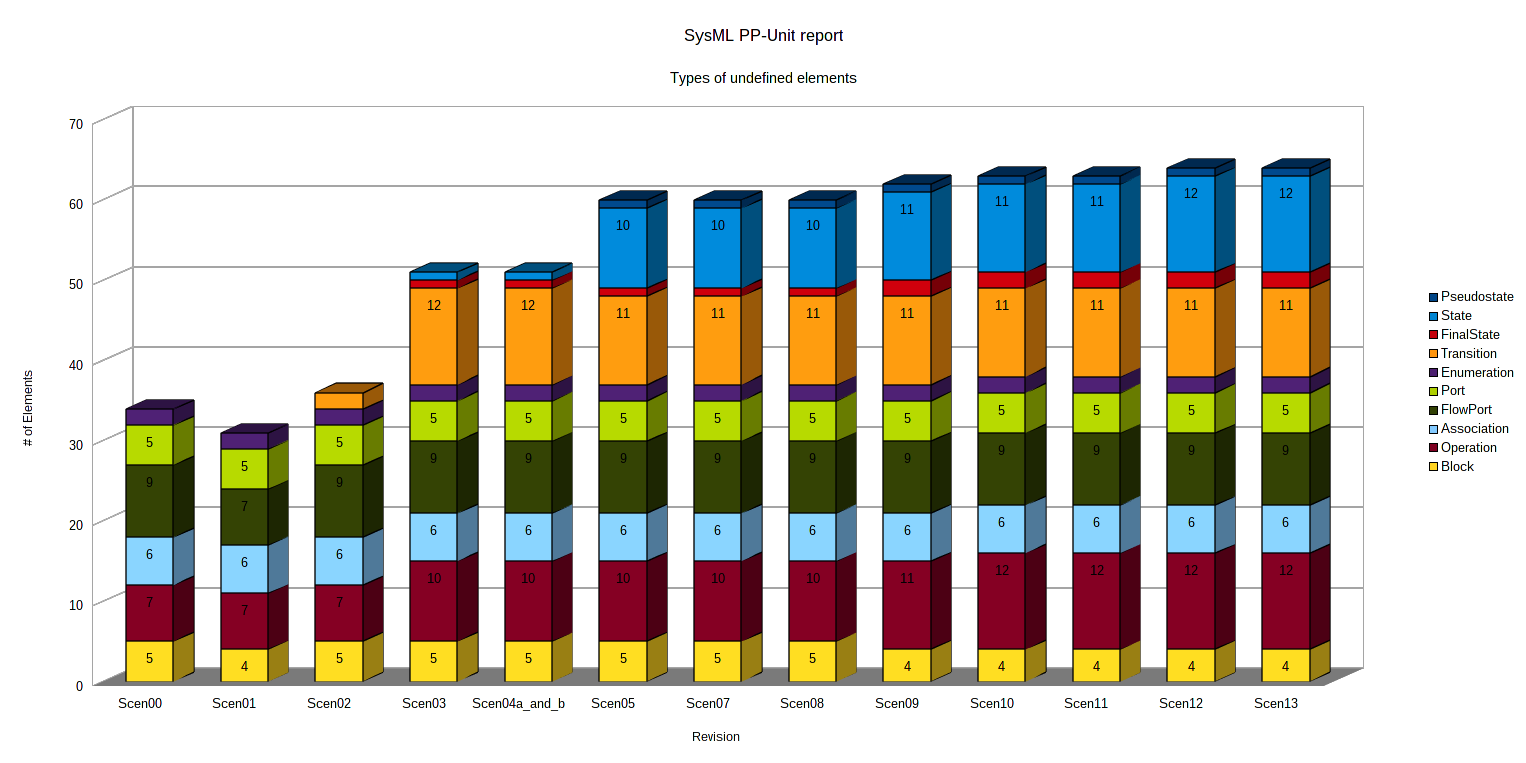
\includegraphics[scale=0.35]{undefinedElementTypes}\\
	\end{center}
	\caption{Types of undefined elements}
	\label{undefinedElementTypes}
	\end{figure} 
	\newpage
  \item \textbf{Hidden model diagrams}\\
  		Hiding elements is not restricted to modeling elements as Papyrus provides
  		the feature of hiding particular diagrams at once. This leads to the same
  		problems described beforehand, whereas in this case more elements are
  		affected at one time. 
\end{itemize}



\section{Adaptions}\label{sysml:adaptions}
As described in the previous section, there have been found different
issues concerning the analyzed \ac{SysML} case study. Both technical and pragmatical
issues have been fixed in the course of this Master's Thesis for making all
revisions compliant to modeling tools and easing the understanding of these
models.
\begin{itemize}
   \item \textbf{Wrong \ac{UUID}s}\\
   		 Using the developed SiDiff services described in chapter~\ref{realization}
   		 all wrong \ac{UUID}s have been fixed and therefore no longer present a
   		 problem to modeling tools relying on identifiers.
   \item \textbf{Usage of EAnnotations}\\
    	 All used EAnnotations concerning tool specific information have been
    	 removed, as they may cause wrong results and do not provide any semantics.
   \item \textbf{Usage of special characters}\\
   		 Special characters, which may cause problems with modeling tools, have
   		 been stripped or replaced by semantically equal ones. The special
   		 character \glqq <\grqq\ has been replaced by the string \glqq
   		 LESSTHAN\grqq\ if this has been the desired semantics of this character
   		 for example.
   \item \textbf{Missing elements}\\
   		 All elements defined as global have been added to the Papyrus diagram
   		 view, so developers can understand the models themselves more easily.
   		 Global elements have not been added, as they may be defined elsewhere.
   \item \textbf{Hidden model diagrams}\\
   		 In the course of this Master's Thesis all hidden diagrams have been
   		 restored and can therefore be used and edited again.
\end{itemize}

After adapting the \ac{PPU} without altering the semantics of said models, the
case study presented in this chapter does not pose a problem to modeling tools
at all. The modified study has been used as exemplary input for all tools and
services created in the course of this Master's Thesis whereas the results are
presented in the following chapter.